\documentclass[tikz]{standalone}

\usepackage{xcolor}
\definecolor{stgoblue}{RGB}{74,144,226}
\definecolor{stgogreen}{RGB}{80,227,194}
\definecolor{stgored}{RGB}{255,69,0}
\definecolor{stgoorange}{RGB}{255,165,0}

\usetikzlibrary{positioning}

\begin{document}

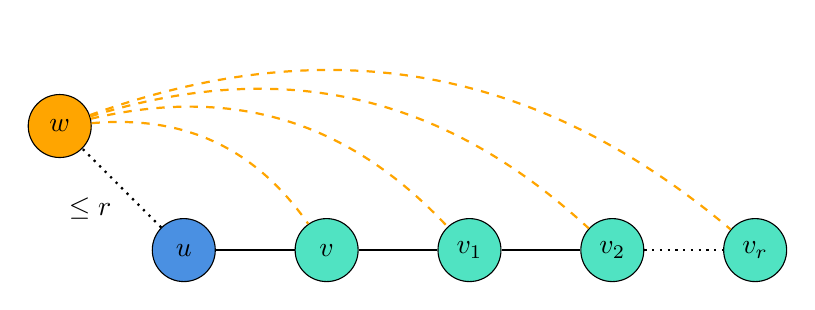
\begin{tikzpicture}
    % Define styles for nodes and edges
    \tikzstyle{node_style}=[circle, draw, inner sep=2pt, minimum size=8mm]
    \tikzstyle{edge_style}=[draw, thick, -]

    % Place nodes
    \node[node_style,fill=stgoblue] (u) {$u$};
    \node[node_style,fill=stgogreen,right=of u] (v) {$v$};
    \node[node_style,fill=stgoorange,above left=of u] (w) {$w$};

    % Place path nodes (v1, v2, ..., vr)
    \node[node_style,fill=stgogreen,right=of v] (v1) {$v_1$};
    \node[node_style,fill=stgogreen,right=of v1] (v2) {$v_2$};
    \node[node_style,fill=stgogreen,right=of v2] (vr) {$v_r$};

    % Connect the nodes with edges
    \draw[edge_style] (u) -- (v);
    \draw[edge_style,dotted] (u) edge node [below left] {$\le r$} (w);
    \draw[edge_style] (v) -- (v1);
    \draw[edge_style] (v1) -- (v2);
    \draw[edge_style,dotted] (v2) -- (vr);

    % Connect w to v, v1, v2, vr with increasing length dashed lines
    \draw[edge_style, dashed, stgoorange] (w) to[bend left] (v);
    \draw[edge_style, dashed, stgoorange] (w) to[bend left] (v1);
    \draw[edge_style, dashed, stgoorange] (w) to[bend left] (v2);
    \draw[edge_style, dashed, stgoorange] (w) to[bend left] (vr);
\end{tikzpicture}

\end{document}
